\documentclass{article}
\usepackage{arxiv}
%\usepackage{amsthm}
\usepackage{amssymb}
\usepackage[utf8]{inputenc} % allow utf-8 input
\usepackage[T1]{fontenc}    % use 8-bit T1 fonts
\usepackage{mathtools}
\usepackage{hyperref}  
\usepackage{mathrsfs}

\usepackage{graphicx}
\usepackage{subcaption}
% hyperlinks
\usepackage{url}            % simple URL typesetting
\usepackage{booktabs}       % professional-quality tables
\usepackage{amsfonts}       % blackboard math symbols
\usepackage{nicefrac}       % compact symbols for 1/2, etc.
\usepackage{microtype}      % microtypography
\usepackage{graphicx}
\usepackage{natbib}
\usepackage{doi}
\usepackage{amsmath}
\usepackage{physics}
\usepackage{wrapfig}
\usepackage{bm}
\usepackage{algorithm,algpseudocode}
\usepackage{xcolor}
\usepackage{forest}
\usepackage{tcolorbox}
\usepackage{tikz-cd}
\usepackage{enumitem}


\newenvironment{proof}{\paragraph{Proof:}}{\hfill$\square$}
\newenvironment{solution}{\paragraph{Solution:}}{\hfill$\square$}


%—– Blackboard‐bold sets —–
\newcommand{\R}{\mathbb{R}}
\newcommand{\N}{\mathbb{N}}
\newcommand{\Z}{\mathbb{Z}}
\newcommand{\Q}{\mathbb{Q}}
\newcommand{\C}{\mathbb{C}}

%—– Probability & expectation —–
\newcommand{\Prb}{\mathbb{P}}        % probability
\newcommand{\E}{\mathbb{E}}           % expectation
\newcommand{\Var}{\mathrm{Var}}       % variance
\newcommand{\Cov}{\mathrm{Cov}}       % covariance

%—– Common math operators —–
\newcommand{\diag}{\operatorname{diag}}
\newcommand{\supp}{\operatorname{supp}}
\newcommand{\argmax}{\operatorname*{arg\,max}}
\newcommand{\argmin}{\operatorname*{arg\,min}}
\newcommand{\ind}{\mathbf{1}}         % indicator

%—– Norms, inner products, absolute value —–

\newcommand{\inner}[2]{\left\langle #1, #2 \right\rangle}

%—– Calligraphic sets —–
\newcommand{\cA}{\mathcal{A}}
\newcommand{\cS}{\mathcal{S}}
\newcommand{\cT}{\mathcal{T}}
\newcommand{\cF}{\mathcal{F}}
\newcommand{\cE}{\mathcal{E}}

%—– RL / MDP notation —–
\newcommand{\SSS}{\mathcal{S}}        % state space
\newcommand{\AAA}{\mathcal{A}}        % action space
\newcommand{\PP}{\mathcal{P}}         % transition kernel
\newcommand{\RRR}{\mathcal{R}}        % reward function
\newcommand{\gammaRL}{\gamma}         % discount factor

%—– Confidence bounds —–
\newcommand{\olQ}{\overline{Q}}
\newcommand{\ulQ}{\underline{Q}}
\newcommand{\olV}{\overline{V}}
\newcommand{\ulV}{\underline{V}}

%—– Miscellaneous —–
\newcommand{\eps}{\varepsilon}
\newcommand{\dt}{\mathrm{d}t}
\newcommand{\given}{\,\bigl\vert\,}    % conditioning bar

%—– Shorthand for frequently used fractions —–
\newcommand{\half}{\tfrac12}
\newcommand{\thalf}{\tfrac32}

%—– Project-specific shorthands —–
\newcommand{\Xs}{\mathcal{X}_s}
\newcommand{\Xu}{\mathcal{X}_u}
\newcommand{\Lie}[2]{\mathcal{L}_{#1} #2}
\newcommand{\hf}{\hat{f}}
\newcommand{\Vol}{\operatorname{Vol}}
\newcommand{\Dict}{\Theta}

%—– Styling —–
\newcommand{\todo}[1]{\textcolor{red}{[TODO: #1]}}


\newcommand{\note}[1]{\begin{tcolorbox}
\textbf{Note:} #1\end{tcolorbox}}

\newtheorem{theorem}{Theorem}
\newtheorem{proposition}[theorem]{Proposition}
\newtheorem{lemma}[theorem]{Lemma}
\newtheorem{corollary}[theorem]{Corollary}
\newtheorem{definition}[theorem]{Definition}
\newtheorem{assumption}[theorem]{Assumption}
\newtheorem{remark}[theorem]{Remark}
\newtheorem{example}[theorem]{Example}
\newtheorem{conjecture}[theorem]{Conjecture}

\title{Lyapunov-Guided Diffusion Control with Learned Dynamics:\\
A Convergence Guarantee under Sparse System Identification}
\date{} 					% Or removing it

\author{ \href{https://orcid.org/0000-0003-1700-756X}{William Chang} \\
	Department of Applied Mathematics\\
	University of California, Los Angeles\\
	Los Angeles, CA \\
	\url{https://williamc.me/} \\
	%% examples of more authors
	\And
}

% Uncomment to override  the `A preprint' in the header
\renewcommand{\headeright}{}
\renewcommand{\undertitle}{}
%\renewcommand{\shorttitle}{\textit{arXiv} Template}

%%% Add PDF metadata to help others organize their library
\hypersetup{
pdftitle={Lyapunov-Guided Diffusion Control with Learned Dynamics},
pdfsubject={},
pdfauthor={William Chang},
pdfkeywords={},
}

\begin{document}
\maketitle
\begin{abstract}
Lyapunov-guided diffusion control synthesizes safe and stable policies by
learning a control Lyapunov--barrier function (CLBF) and using it to guide a
diffusion-based trajectory sampler. The certificate certifies stability through
its decrease along the system trajectories, which couples it to the vector field
$f$ of the controlled dynamical system. Existing analyses, however, treat $f$ as
\emph{known}: the dissipation of the certificate is evaluated against the true
dynamics, and convergence holds up to a small ``bad set'' on which dissipation is
allowed to fail. In many settings the dynamics are not available and one observes
only trajectory data. We study the data-driven regime in which $f$ is first
estimated from observed transitions by sparse identification of nonlinear
dynamics (SINDy), and the certificate is then trained and the diffusion sampler
guided against the \emph{estimated} field $\hf$. Our main result shows that the
true closed-loop system still converges almost surely to a neighbourhood of the
goal, and that the estimation enters the bound through a single additive term
proportional to the dynamics error $\delta=\|f-\hf\|_\infty$. Concretely, the
certificate satisfies $V(x_t)\le e^{-\lambda_1 t}V(x_0)+C\eps^{1/n}+B\delta/\lambda_1$,
where $\eps$ bounds the volume of the bad set and $B$ bounds $\|\nabla V\|$. The
guarantee degrades gracefully in $\delta$ and recovers the known-dynamics result
of \citet{cheng2026safe} as $\hf\to f$; a corollary relates $\delta$ to the
recovery error of the sparse coefficients.
\end{abstract}


\section{Introduction}

Safe and stable control asks for policies that keep a system inside a prescribed
safe region while driving its state toward a goal. A classical and flexible way
to encode both requirements is through a \emph{certificate}: a scalar function of
the state whose sublevel sets describe safe configurations and whose decrease
along trajectories witnesses convergence. Control Lyapunov functions, control
barrier functions, and their combination into control Lyapunov--barrier functions
(CLBFs) are the standard instances. The defining property is not the geometry of
the level sets alone, but the \emph{dissipation} condition: along the trajectories
generated by the closed-loop dynamics, the certificate must decrease, typically at
a rate proportional to its current value.

Recent work on Lyapunov-guided diffusion couples this idea with generative
trajectory planning. \citet{cheng2026safe} learn a CLBF and use it to guide a
diffusion sampler over control sequences, so that sampled trajectories are biased
toward low cost, safe states, and decreasing certificate values. A central
observation of that work is that the learned certificate need not dissipate
\emph{everywhere}: drawing on almost-Lyapunov theory, they show that if the
dissipation condition can fail only on a set $\Omega$ of small volume, the
system still converges to a small neighbourhood of the goal, with the size of the
neighbourhood controlled by $\Vol(\Omega)$. This tolerance is what makes
\emph{learned} certificates usable, since a finite sample can never certify
dissipation at every point of a continuum.

These guarantees are stated for a \emph{known} vector field. The dissipation is
the Lie derivative $\Lie{f}{V}(x,u)=\nabla V(x)^\top f(x,u)$, which presupposes
access to $f$; the diffusion sampler likewise rolls out candidate trajectories
through $f$. This is natural for the physical control tasks used as benchmarks,
where the equations of motion of a pendulum or a tracking vehicle are available
in closed form. In many practical settings the dynamics are unknown and one has
only a record of how the state responded to applied controls, that is, a dataset
of transitions $\{(x_i,u_i,x_i^+)\}$. The question we study is whether the
Lyapunov-guided diffusion guarantee survives when $f$ must first be estimated
from such data.

We answer this affirmatively for vector fields that are sparse in a chosen
dictionary of features. We estimate $f$ by sparse identification of nonlinear
dynamics \citep{brunton2016discovering}: from the transition data we form
derivative estimates, regress them on a library of candidate functions of the
state and control, and select a parsimonious model by an $\ell_1$-penalized fit.
The certificate is then trained, and the diffusion sampler guided, against the
estimated field $\hf$ rather than the unknown $f$. Our contribution is a
convergence analysis for the \emph{true} closed-loop system under this learned
model. The estimation error enters the bound through a single additive term: with
$\delta=\|f-\hf\|_\infty$ the worst-case vector-field error and $B$ a bound on
$\|\nabla V\|$, the certificate obeys
\[
    V(x_t)\;\le\; e^{-\lambda_1 t}\,V(x_0)\;+\;C\,\eps^{1/n}\;+\;\frac{B\,\delta}{\lambda_1},
    \qquad \forall t\ge 0,
\]
almost surely, where $\eps$ bounds $\Vol(\Omega)$ and $n=\dim\mathcal{X}$. The two
non-transient terms have clean interpretations: $C\eps^{1/n}$ is the price of
allowing the certificate to misbehave on the bad set, exactly as in the
known-dynamics analysis, and $B\delta/\lambda_1$ is the price of acting on an
estimated model. The bound degrades gracefully in $\delta$ and collapses to the
result of \citet{cheng2026safe} as $\hf\to f$. A corollary translates $\delta$
into the recovery error of the sparse coefficients, so that consistent
identification yields the original guarantee in the limit.

\section{Preliminaries}

\subsection{Controlled dynamical systems}

Let $\mathcal{X}\subseteq\R^n$ be a compact state space and
$\mathcal{U}\subseteq\R^m$ a compact control space. We consider a controlled,
continuous-time system
\begin{equation}
\label{eq:dynamics}
    \dot{x}(t) \;=\; f\bigl(x(t),u(t)\bigr),
    \qquad x(t)\in\mathcal{X},\; u(t)\in\mathcal{U},
\end{equation}
where $f:\mathcal{X}\times\mathcal{U}\to\R^n$ is globally Lipschitz. A goal state
$x_\star\in\Xs$ and a safe set $\Xs\subseteq\mathcal{X}$ (with unsafe complement
$\Xu=\mathcal{X}\setminus\Xs$) are given; the safe set may be described by
constraints $\Xs=\{x:g_j(x)\le 0,\ j=1,\dots,J\}$ or by labels. A control signal
induces a trajectory $\{x(t),u(t)\}_{t\ge 0}$, and the trajectory is safe if
$x(t)\in\Xs$ for all $t\ge 0$. The aim of safe and stable control is to keep the
state in $\Xs$ while driving it to $x_\star$.

In the data-driven setting we do not have $f$. Instead we observe a dataset of
transitions sampled at period $\Delta t>0$,
\begin{equation}
\label{eq:data}
    \mathcal{D} \;=\; \bigl\{(x_i,u_i,x_i^+)\bigr\}_{i=1}^N,
\end{equation}
where $x_i^+$ is the state observed after applying $u_i$ at $x_i$. Finite
differences yield derivative estimates
\begin{equation}
\label{eq:fd}
    \dot{x}_i \;\approx\; \frac{x_i^+ - x_i}{\Delta t},
\end{equation}
which are accurate to first order in $\Delta t$ for smooth dynamics.

\subsection{Control Lyapunov--barrier functions}

We use the certificate of \citet{cheng2026safe}, which simultaneously encodes
safety and stability.

\begin{definition}[CLBF]
\label{def:clbf}
A continuously differentiable function $V:\mathcal{X}\to\R_{\ge 0}$ is a control
Lyapunov--barrier function for constants $c,\lambda>0$ if
\begin{align}
\text{(equilibrium)}\quad & V(x_\star)=0, \label{eq:clbf-eq}\\
\text{(positivity)}\quad & V(x)>0, \quad \forall x\in\mathcal{X}\setminus\{x_\star\}, \label{eq:clbf-pos}\\
\text{(safe set)}\quad & V(x)\le c, \quad \forall x\in\Xs, \label{eq:clbf-safe}\\
\text{(unsafe set)}\quad & V(x)>c, \quad \forall x\in\mathcal{X}\setminus\Xs, \label{eq:clbf-unsafe}\\
\text{(dissipation)}\quad & \inf_{u\in\mathcal{U}} \Lie{f}{V}(x,u)+\lambda V(x)\le 0,
    \quad \forall x\in\mathcal{X}\setminus\{x_\star\}, \label{eq:clbf-diss}
\end{align}
where $\Lie{f}{V}(x,u)=\nabla V(x)^\top f(x,u)$ is the Lie derivative of $V$ along
$f$.
\end{definition}

Conditions \eqref{eq:clbf-safe}--\eqref{eq:clbf-unsafe} make the sublevel set
$\{V\le c\}$ coincide with the safe region, while the dissipation condition
\eqref{eq:clbf-diss} forces $V$ to decrease along trajectories at an exponential
rate. When $V$ is a genuine CLBF, the closed loop is exponentially stable:
$V(x_t)\le e^{-\lambda t}V(x_0)$, and $x_\star$ is reached while $\{V\le c\}$ is
never left.

\subsection{Almost-Lyapunov certificates and the known-dynamics guarantee}

A learned certificate cannot be expected to satisfy \eqref{eq:clbf-diss}
pointwise everywhere. Almost-Lyapunov theory relaxes the requirement to a set of
full measure up to a small exception. Let $\Omega\subset\mathcal{X}$ be a
measurable ``bad set'' on which dissipation may fail. The following regularity
conditions, adopted from \citet{cheng2026safe}, are used throughout.

\begin{assumption}[Regularity]
\label{ass:reg}
The sets $\mathcal{X},\mathcal{U}$ are compact, $f$ is globally Lipschitz, and the
candidate certificate $V\in C^2(\mathcal{X})$ has uniformly bounded gradient and
Hessian and bounded dynamics:
\[
    \|\nabla V\|_\infty\le B,\qquad
    \|\nabla^2 V\|_\infty\le B,\qquad
    \|f\|_\infty\le B,\qquad
    \|\nabla f\|_\infty\le B,
\]
for some constant $B>0$. The control policy $u(\cdot)$ is Lipschitz in the state.
\end{assumption}

The convergence guarantee for known dynamics rests on the standard comparison
(Gr\"onwall) inequality, which we record for later use.

\begin{lemma}[Comparison inequality]
\label{lem:comparison}
Let $V_t:=V(x_t)$ be continuously differentiable and satisfy
$\dot V_t\le -\lambda V_t + C$ for all $t\ge 0$, with $\lambda>0$ and $C\in\R$.
Then
\[
    V_t \;\le\; e^{-\lambda t}\,V_0 \;+\; \frac{C}{\lambda}\bigl(1-e^{-\lambda t}\bigr)
    \;\le\; e^{-\lambda t}\,V_0 \;+\; \frac{C}{\lambda}.
\]
\end{lemma}

\citet{cheng2026safe} combine Lemma~\ref{lem:comparison} with a martingale
argument for the diffusion-sampled policy to obtain the following guarantee, which
our main result extends to learned dynamics.

\begin{theorem}[Known-dynamics guarantee, \citealp{cheng2026safe}]
\label{thm:known}
Let Assumption~\ref{ass:reg} hold, and suppose there exist $\lambda>0$,
$\eps>0$, and a connected, measurable, invariant bad set $\Omega\subset\mathcal{X}$
with $\Vol(\Omega)<\eps$ such that
\begin{enumerate}[label=\textnormal{(\Alph*)},leftmargin=2.4em]
    \item for every $x\in\mathcal{X}\setminus\Omega$,
    $\displaystyle \min_{u\in\mathcal{U}}\Lie{f}{V}(x,u)\le -\lambda V(x)$;
    \item for $x\in\Omega$, no dissipation condition is imposed.
\end{enumerate}
Then there exist constants $\lambda_1\in(0,\lambda)$ and $C>0$ such that, for any
$x_0\in\Xs$, the solution of \eqref{eq:dynamics} under the diffusion-sampled
policy satisfies, almost surely,
\begin{equation}
\label{eq:known-bound}
    V(x_t)\;\le\; e^{-\lambda_1 t}\,V(x_0) \;+\; C\,\eps^{1/n},
    \qquad \forall t\ge 0.
\end{equation}
\end{theorem}

The bad set contributes only the additive term $C\eps^{1/n}$, so the trajectory
contracts to the sublevel set $\{V\le C\eps^{1/n}\}$ up to transient exponential
decay.

\subsection{Diffusion-guided trajectory sampling}

The policy that realizes the dissipation in practice is obtained by guided
diffusion. Over a horizon $T$, a candidate control sequence $U_{1:T}=(u_1,\dots,u_T)$
is drawn from an unnormalized trajectory distribution
\[
    p(U_{1:T}\mid x_0)\;\propto\;
    \exp\!\Bigl(-\tfrac{1}{\gamma_1}\textstyle\sum_t q(x_t,u_t)\Bigr)\,
    \prod_t \ind\{V(x_t)\le c\}\,
    \exp\!\Bigl(-\tfrac{1}{\gamma_2}\textstyle\sum_t \bigl\|[\,\Lie{f}{V}(x_t,u_t)+\lambda V(x_t)\,]_+\bigr\|^2\Bigr),
\]
where $q$ is the task cost, $[z]_+=\max\{z,0\}$, and $\gamma_1,\gamma_2>0$ are
temperatures. The three factors bias samples toward low cost, the safe sublevel
set, and certificate decrease, respectively. The crucial point for us is that both
the rollout $x_{t+1}\approx x_t+\Delta t\,f(x_t,u_t)$ and the stability factor are
evaluated through $f$; replacing $f$ by an estimate is precisely the modification
we analyze.

\section{Main result: certificate-guided control under learned dynamics}

We now remove the assumption that $f$ is known. The plan is: (i) estimate $f$ from
the transition data \eqref{eq:data} by sparse identification; (ii) train the CLBF
and guide the diffusion sampler against the estimate $\hf$; and (iii) bound the
behaviour of the \emph{true} system \eqref{eq:dynamics} in closed loop.

\subsection{Sparse identification of the dynamics}

We estimate $f$ by sparse identification of nonlinear dynamics
\citep{brunton2016discovering}. The premise is that, although $f$ may be
nonlinear, in suitable coordinates it is governed by only a handful of terms,
i.e.\ it is \emph{sparse} in a sufficiently rich dictionary of candidate
features. The procedure has three parts: forming the data and its derivatives,
choosing the feature library, and solving a sparse regression for the coefficients.

\paragraph{Data and derivatives.}
From the transitions \eqref{eq:data} we assemble two matrices whose rows are the
$N$ sampled snapshots,
\[
    X = \begin{bmatrix} x_1^\top\\ \vdots\\ x_N^\top \end{bmatrix}\in\R^{N\times n},
    \qquad
    \dot X = \begin{bmatrix} \dot x_1^\top\\ \vdots\\ \dot x_N^\top \end{bmatrix}\in\R^{N\times n},
    \qquad
    U = \begin{bmatrix} u_1^\top\\ \vdots\\ u_N^\top \end{bmatrix}\in\R^{N\times m},
\]
with the controls stacked alongside. When only states are measured, the
derivatives $\dot X$ are obtained by differentiation. The naive finite difference
\eqref{eq:fd} carries an $\mathcal{O}(\Delta t)$ truncation bias and, more
importantly, \emph{amplifies measurement noise}; following
\citet{brunton2016discovering} we therefore recommend computing $\dot X$ by
total-variation regularized differentiation, which denoises the derivative and
makes the identification markedly more robust than direct differencing.

\paragraph{Feature library.}
Fix a dictionary of $p$ candidate functions of the state and control, evaluated
row-wise on the data,
\[
    \Dict(X,U)=
    \bigl[\, \mathbf{1}\ \ X\ \ X^{P_2}\ \ X^{P_3}\ \ \cdots\ \ \sin(X)\ \ \cos(X)\ \ \cdots\ \ U\ \ \cdots \,\bigr]
    \;\in\;\R^{N\times p},
\]
where $\mathbf{1}$ is the constant column, $X$ the linear terms, and $X^{P_2}$ the
block of quadratic monomials in the state,
\[
    X^{P_2}=\bigl[\,x_1^2,\ x_1 x_2,\ \dots,\ x_1 x_n,\ x_2^2,\ \dots,\ x_n^2\,\bigr],
\]
with higher polynomial and trigonometric blocks defined analogously, and control
features (and state--control products) appended to cover forced systems
\citep{brunton2016discovering}. We write $\Dict(x,u)\in\R^{1\times p}$ for the
same features evaluated at a single point $(x,u)$. The choice of coordinates and
library is the one modelling decision the method requires: the dynamics are sparse
only in an appropriate basis, and prior physical knowledge (e.g.\ that mechanical
systems carry trigonometric and polynomial terms) guides its construction. We take
$p\ll N$, so the regression below is overdetermined.

\paragraph{Sparse regression.}
The dictionary turns identification into a linear-in-parameters problem: with a
coefficient matrix $\Xi\in\R^{p\times n}$,
\begin{equation}
\label{eq:sindy-model}
    \dot X \;=\; \Dict(X,U)\,\Xi \;+\; \eta Z,
\end{equation}
where $\eta Z$ collects measurement and derivative noise. Crucially, the $n$ state
equations \emph{decouple}: column $k$ of \eqref{eq:sindy-model} reads
$\dot X_{:,k}\approx \Dict(X,U)\,\xi_k$, so each $\xi_k\in\R^{p}$ is found by a
separate scalar regression and a different equation may select a different set of
active terms. Sparsity of $\xi_k$ encodes the principle that few features govern
each component of the dynamics; it is what keeps the model parsimonious and lets
it extrapolate beyond the sampled region rather than overfit it. We solve for the
sparse coefficients in one of two equivalent ways. The first is an
$\ell_1$-penalized (LASSO) regression,
\begin{equation}
\label{eq:sindy}
    \hat\Xi \;=\; \argmin_{\Xi\in\R^{p\times n}}
    \;\frac{1}{N}\bigl\|\dot X-\Dict(X,U)\,\Xi\bigr\|_F^2
    \;+\;\kappa\,\|\Xi\|_1,
    \qquad \|\Xi\|_1=\textstyle\sum_{j,k}|\Xi_{jk}|,
\end{equation}
with $\kappa>0$ controlling the degree of sparsity. The second, often cheaper and
governed by a single threshold $\lambda$, is the sequentially thresholded
least-squares (STLSQ) procedure of \citet{brunton2016discovering}, which
alternates an ordinary least-squares fit with the elimination of small
coefficients until the active set stabilizes (Algorithm~\ref{alg:stlsq}).

\begin{algorithm}[t]
\caption{Sequentially thresholded least squares (STLSQ) \citep{brunton2016discovering}}
\label{alg:stlsq}
\begin{algorithmic}[1]
\State \textbf{Input:} feature matrix $\Dict=\Dict(X,U)\in\R^{N\times p}$, derivatives $\dot X\in\R^{N\times n}$, threshold $\lambda>0$
\State $\Xi \gets \Dict^{\dagger}\dot X$ \Comment{initial least-squares fit; $\Dict^\dagger$ is the pseudoinverse}
\Repeat
    \State $\Xi_{jk}\gets 0$ for all $(j,k)$ with $|\Xi_{jk}|<\lambda$ \Comment{threshold small coefficients}
    \For{$k=1,\dots,n$} \Comment{refit each state equation on its active terms}
        \State $J_k\gets\{\,j:\Xi_{jk}\neq 0\,\}$
        \State $\Xi_{J_k,k}\gets \Dict(:,J_k)^{\dagger}\,\dot X_{:,k}$
    \EndFor
\Until{the active set $\{(j,k):\Xi_{jk}\neq 0\}$ stops changing}
\State \textbf{return} $\hat\Xi \gets \Xi$
\end{algorithmic}
\end{algorithm}

The recovered vector field is read off from the coefficients,
\begin{equation}
\label{eq:fhat}
    \hf(x,u)\;=\;\hat\Xi^\top\,\Dict(x,u)^\top \;\in\;\R^n,
\end{equation}
which is the analytic model used everywhere downstream: its gradient
$\nabla_x\hf$ is available in closed form for the Lie-derivative penalty, and it is
integrated to roll out trajectories inside the diffusion sampler.

\paragraph{From estimate to error.}
We summarize the quality of $\hf$ by the worst-case vector-field error over the
operating region,
\begin{equation}
\label{eq:delta}
    \delta \;:=\; \sup_{(x,u)\in\mathcal{X}\times\mathcal{U}} \bigl\|f(x,u)-\hf(x,u)\bigr\|_2.
\end{equation}
Three sources feed $\delta$: the truncation bias of the derivative estimate
\eqref{eq:fd}, of order $\mathcal{O}(\Delta t)$ for smooth $f$ (mitigated by the
total-variation derivative above); the statistical error of the regression
\eqref{eq:sindy} from finite, noisy data; and any \emph{misspecification} bias if
$f$ is not exactly representable in the chosen library. When the library is rich
enough that $f$ lies in its span, the first two sources dominate and $\delta$ is
governed entirely by the recovery error of the coefficients $\hat\Xi$, which we
make precise in Corollary~\ref{cor:coeff}. The quantity $\delta$ is the only
property of the identification step that enters our convergence guarantee.

\subsection{Certificate learning against the estimated dynamics}

With $\hf$ in hand we replace every occurrence of $f$ in the certificate and the
sampler by its estimate. The estimated Lie derivative is
\[
    \Lie{\hf}{V}(x,u)\;=\;\nabla V(x)^\top \hf(x,u),
\]
and the CLBF is trained by minimizing, over a parameterized $V_\phi$, the empirical
risk
\[
\begin{aligned}
    \mathcal{L}(\phi)=\E_{x\sim\mathcal{D}}\Bigl[\;
    &\ind_{\{x=x_\star\}}\|V_\phi(x)\|
    +[-V_\phi(x)]_+
    +\ind_{\{x\in\Xs\}}[V_\phi(x)-c]_+
    +\ind_{\{x\notin\Xs\}}[c-V_\phi(x)]_+\\
    &+\alpha\,\bigl[\Lie{\hf}{V_\phi}(x,u)+\lambda V_\phi(x)+\eps_0\bigr]_+
    \;\Bigr],
\end{aligned}
\]
where $\alpha>0$ weights the dissipation term and $\eps_0\ge 0$ is a robustness
margin. The first four terms enforce the equilibrium, positivity, and
safe/unsafe conditions \eqref{eq:clbf-eq}--\eqref{eq:clbf-unsafe}; the last term
enforces dissipation \emph{against the estimated field}. The diffusion sampler is
modified identically, rolling out $x_{t+1}\approx x_t+\Delta t\,\hf(x_t,u_t)$ and
penalizing $[\Lie{\hf}{V}(x_t,u_t)+\lambda V(x_t)]_+$. Training therefore certifies
\begin{equation}
\label{eq:est-diss}
    \min_{u\in\mathcal{U}}\Lie{\hf}{V}(x,u)\;\le\;-\lambda V(x),
    \qquad \forall x\in\mathcal{X}\setminus\Omega,
\end{equation}
for some bad set $\Omega$ of small volume, exactly as in
Theorem~\ref{thm:known} but with $\hf$ in place of $f$. The gap between
\eqref{eq:est-diss} and the dissipation that actually governs the true trajectory
is the entire content of the analysis below.

\subsection{Convergence under estimated dynamics}

The trajectory evolves under the true $f$, yet dissipation is certified only for
$\hf$. The next lemma converts the estimated condition \eqref{eq:est-diss} into a
true dissipation condition with an additive slack proportional to $\delta$.

\begin{lemma}[Dissipation transfer]
\label{lem:transfer}
Under Assumption~\ref{ass:reg}, suppose $V$ satisfies the estimated dissipation
condition \eqref{eq:est-diss} on $\mathcal{X}\setminus\Omega$, and let
$\delta$ be as in \eqref{eq:delta}. Then, along the true dynamics
\eqref{eq:dynamics}, for every $x\in\mathcal{X}\setminus\Omega$ and the
corresponding control $u$,
\[
    \Lie{f}{V}(x,u)\;\le\;-\lambda V(x) + B\,\delta.
\]
\end{lemma}

\begin{proof}
Split the true Lie derivative into the estimated part and a residual, and apply
Cauchy--Schwarz with the gradient bound from Assumption~\ref{ass:reg}:
\[
    \Lie{f}{V}(x,u)
    =\nabla V(x)^\top f(x,u)
    =\underbrace{\nabla V(x)^\top \hf(x,u)}_{=\,\Lie{\hf}{V}(x,u)}
    +\nabla V(x)^\top\bigl(f(x,u)-\hf(x,u)\bigr).
\]
The first term is at most $-\lambda V(x)$ by \eqref{eq:est-diss}. The second is
bounded by $\|\nabla V(x)\|\,\|f(x,u)-\hf(x,u)\|\le B\,\delta$ using
\eqref{eq:delta}. Adding the two estimates gives the claim.
\end{proof}

We can now state the convergence guarantee for the data-driven scheme. It is the
analogue of Theorem~\ref{thm:known} in which the certified field is $\hf$ and the
true field is $f$.

\begin{theorem}[Convergence under learned dynamics]
\label{thm:main}
Let Assumption~\ref{ass:reg} hold, let $\hf$ be the estimated field
\eqref{eq:fhat} with error $\delta$ as in \eqref{eq:delta}, and suppose there
exist $\lambda>0$, $\eps>0$, and a connected, measurable, invariant bad set
$\Omega\subset\mathcal{X}$ with $\Vol(\Omega)<\eps$ such that the estimated
dissipation \eqref{eq:est-diss} holds on $\mathcal{X}\setminus\Omega$ and no
condition is imposed on $\Omega$. Then there exist constants $\lambda_1\in(0,\lambda)$
and $C>0$, independent of $\delta$, such that for any $x_0\in\Xs$ the solution of
the true system \eqref{eq:dynamics} under the diffusion-sampled policy satisfies,
almost surely,
\begin{equation}
\label{eq:main-bound}
    V(x_t)\;\le\; e^{-\lambda_1 t}\,V(x_0)
    \;+\; C\,\eps^{1/n}
    \;+\; \frac{B\,\delta}{\lambda_1},
    \qquad \forall t\ge 0.
\end{equation}
Consequently $\displaystyle \limsup_{t\to\infty} V(x_t)\le C\,\eps^{1/n}+B\delta/\lambda_1$
almost surely, i.e.\ the true trajectory contracts to the sublevel set
$\{\,V\le C\eps^{1/n}+B\delta/\lambda_1\,\}$.
\end{theorem}

\begin{proof}
By Lemma~\ref{lem:transfer}, the estimated dissipation \eqref{eq:est-diss}
implies that along the true dynamics
\[
    \Lie{f}{V}(x,u)\le -\lambda V(x)+B\delta,
    \qquad \forall x\in\mathcal{X}\setminus\Omega.
\]
This is exactly the hypothesis of the known-dynamics analysis of
Theorem~\ref{thm:known}, except that the right-hand side carries the constant
slack $B\delta$. We follow that argument in two steps.

\emph{Step 1 (uniform slack-dissipation outside a small neighbourhood).}
Inflate the bad set to its $r$-neighbourhood
$\Omega_r=\{x:\operatorname{dist}(x,\Omega)\le r\}$. By Steiner's volume-growth
estimate, $\Vol(\Omega_r)\le \Vol(\Omega)+\mathcal{O}(r)$, so choosing
$r=\mathcal{O}(\eps^{1/n})$ keeps $\Vol(\Omega_r)\le 2\eps$ while recovering, on the
complement $\mathcal{X}\setminus\Omega_r$, the pointwise inequality
$\Lie{f}{V}(x,u)\le -\lambda V(x)+B\delta$. Following \citet{cheng2026safe}, the
contribution of $\Omega_r$ to the certificate along trajectories is bounded by a
term of order $\Vol(\Omega_r)^{1/n}=\mathcal{O}(\eps^{1/n})$, and a rate
$\lambda_1\in(0,\lambda)$ is obtained that absorbs this contribution; this yields
the term $C\eps^{1/n}$ and a differential inequality of the form
\[
    \dot V_t \;\le\; -\lambda_1 V_t + B\delta
\]
that holds along the closed-loop trajectory outside the buffer.

\emph{Step 2 (comparison and almost-sure decay).}
Applying the comparison inequality of Lemma~\ref{lem:comparison} with rate
$\lambda_1$ and constant $C':=B\delta$ gives
\[
    V_t \;\le\; e^{-\lambda_1 t}V_0+\frac{B\delta}{\lambda_1}\bigl(1-e^{-\lambda_1 t}\bigr)
    \;\le\; e^{-\lambda_1 t}V_0+\frac{B\delta}{\lambda_1},
\]
to which the bad-set term $C\eps^{1/n}$ from Step 1 is added. The almost-sure
qualifier and the rate $\lambda_1$ are inherited verbatim from the martingale
concentration argument for the diffusion-sampled policy in
\citet{cheng2026safe}, since the dynamics estimation enters only through the
deterministic slack $B\delta$ and not through the stochasticity of the sampler.
Combining the two steps gives \eqref{eq:main-bound}, and letting $t\to\infty$
gives the $\limsup$ statement.
\end{proof}

\begin{remark}[Recovering the known-dynamics guarantee]
\label{rem:recover}
The bound \eqref{eq:main-bound} differs from the known-dynamics bound
\eqref{eq:known-bound} only by the additive term $B\delta/\lambda_1$. As the
estimate improves, $\delta\to 0$ and \eqref{eq:main-bound} collapses to
\eqref{eq:known-bound}; in particular, if the dictionary contains $f$ and the
regression \eqref{eq:sindy} is consistent, the data-driven scheme attains the
original guarantee in the large-sample limit.
\end{remark}

The final corollary makes the dependence on identification explicit. When the
true field is realizable in the dictionary, the vector-field error $\delta$ is
controlled by the recovery error of the sparse coefficients, which is the natural
output of a sparse-regression consistency analysis.

\begin{corollary}[From coefficient recovery to convergence]
\label{cor:coeff}
Suppose $f(x,u)=\Xi^\top\Dict(x,u)^\top$ for some $\Xi\in\R^{p\times n}$ (dictionary
realizability), and let
$\Dict_{\max}:=\sup_{(x,u)\in\mathcal{X}\times\mathcal{U}}\|\Dict(x,u)\|_2$. Then the
estimate \eqref{eq:fhat} satisfies
$\delta\le \Dict_{\max}\,\|\hat\Xi-\Xi\|_2$, and the steady-state bound of
Theorem~\ref{thm:main} becomes
\[
    \limsup_{t\to\infty} V(x_t)\;\le\; C\,\eps^{1/n}+\frac{B\,\Dict_{\max}}{\lambda_1}\,\|\hat\Xi-\Xi\|_2
    \qquad \text{a.s.}
\]
In particular, consistent identification $\hat\Xi\to\Xi$ drives the offset to
$C\eps^{1/n}$, matching Theorem~\ref{thm:known}.
\end{corollary}

\begin{proof}
For any $(x,u)$, realizability gives
$f(x,u)-\hf(x,u)=(\Xi-\hat\Xi)^\top\Dict(x,u)^\top$, hence
$\|f(x,u)-\hf(x,u)\|_2\le\|\hat\Xi-\Xi\|_2\,\|\Dict(x,u)\|_2\le\Dict_{\max}\|\hat\Xi-\Xi\|_2$.
Taking the supremum over $(x,u)$ bounds $\delta$, and substituting into
\eqref{eq:main-bound} and letting $t\to\infty$ gives the displayed inequality.
\end{proof}

\section{Empirical Validation}
\label{sec:experiments}

The analysis above predicts that replacing the true field $f$ by a
sparse-identified estimate $\hf$ leaves the convergence guarantee intact up to the
additive offset $B\delta/\lambda_1$. We test this end to end on the inverted
pendulum: we (i) collect transition data under the true dynamics, (ii) recover
$\hf$ by SINDy, and (iii) train the CLBF and run the diffusion-guided controller
\emph{entirely against $\hf$}, comparing against an identical pipeline that retains
the true $f$. The implementation reuses the controller of \citet{cheng2026safe}
without modification: only the object supplying $\mathtt{closed\_loop\_dynamics}$
is swapped, so that every certificate evaluation, Lie-derivative penalty, and
diffusion rollout is computed through the estimated model.

\subsection{Setup}
\label{sec:exp-setup}

The system is the torque-controlled inverted pendulum with state
$x=(\theta,\dot\theta)\in\R^2$ and scalar control $u$ (parameters $m=1$, $L=1$,
$b=0.01$). The goal is the upright equilibrium $x_\star=0$, and the safe set is a
box around it. Both the baseline and the data-driven pipeline are trained for
$51$ epochs ($7191$ optimizer steps each) on identical data modules, network
architecture, and optimizer; the only difference is the dynamics object passed to
the controller. To rule out any leakage of true-physics information into the
data-driven pipeline, the nominal/exploration LQR gain $K$ and the associated
Lyapunov matrix $P$ used by the controller are computed entirely from the learned
model $\hf$: we linearize $\hf$ at the goal by central finite differences and
solve the corresponding LQR and Lyapunov equations, so no quantity derived from
the true field $f$ enters certificate synthesis.

\paragraph{Data collection.}
We gather a dataset of $N=20{,}000$ transitions
$\mathcal{D}=\{(x_i,u_i,x_i^+)\}$ by rolling out a conservative exploration policy
under the true dynamics, restricted to the operating region
$\theta\in[-0.50,0.48]$, $\dot\theta\in[-0.59,0.61]$ around the goal. Derivatives
$\dot x_i$ are formed as in \eqref{eq:fd} at $\Delta t=0.01$, yielding the
matrices $X,U,\dot X$ of Section~3.1.

\paragraph{Identification.}
We fit \eqref{eq:sindy-model} with a degree-$3$ polynomial-plus-trigonometric
library ($p=26$ candidate features) by sequentially thresholded least squares
(Algorithm~\ref{alg:stlsq}). The recovered field is
\begin{align*}
    \dot\theta\;&=\;0.507\,\dot\theta + 0.081\,\dot\theta^{3} + 0.493\,\sin\dot\theta,\\
    \ddot\theta\;&=\;4.859\,\theta - 0.025\,\dot\theta + 1.000\,u
        - 0.341\,\theta^{3} + 0.551\,\theta^{2}\dot\theta + 0.011\,\theta\dot\theta^{2}
        - 0.121\,\dot\theta^{3} + 4.915\,\sin\theta.
\end{align*}
The control channel is recovered exactly ($\hat\Xi_{u}=1.000$). The gravity term
is split between the linear and sinusoidal features, whose coefficients sum to
$4.859+4.915\approx 9.77\approx g$; since $\sin\theta\approx\theta$ on the
operating region, the two representations agree there, while the spurious
high-order terms account for the residual. Identification is essentially exact on
the operating region: the coefficient of determination is $R^2=1.000$ for
$\dot\theta$ and $R^2=0.99999$ for $\ddot\theta$, with per-component RMSE of
$1.0\times10^{-5}$ and $2.9\times10^{-3}$ respectively.

\paragraph{Estimated dynamics error.}
Evaluating \eqref{eq:delta} over the operating region (the support of the safe
sublevel set, where the certificate and sampler are queried) gives a worst-case
error $\delta=\sup\|f-\hf\|_2\approx 0.049$, with mean $1.5\times10^{-3}$ and
median $7\times10^{-4}$. The implied offset $B\delta/\lambda_1$ in
Theorem~\ref{thm:main} is therefore small, and we expect the data-driven
certificate to behave almost indistinguishably from the known-dynamics one. (The
error grows under aggressive extrapolation far outside the sampled region, where
the $\dot\theta^{3}$ and $\sin$ decompositions diverge from the identity;
this regime lies outside the safe set and does not enter the guarantee.)

\subsection{Results}
\label{sec:exp-results}

We track the CLBF training loss --- the mean-squared violation of the certificate
conditions \eqref{eq:clbf-eq}--\eqref{eq:clbf-diss}, reported as
\emph{CLBF MSE} --- per epoch for both pipelines. A small CLBF MSE means the
learned $V$ satisfies the equilibrium, positivity, safe/unsafe, and dissipation
conditions almost everywhere; driving it toward zero is exactly the act of
synthesizing a valid certificate.

\begin{figure}[t]
    \centering
    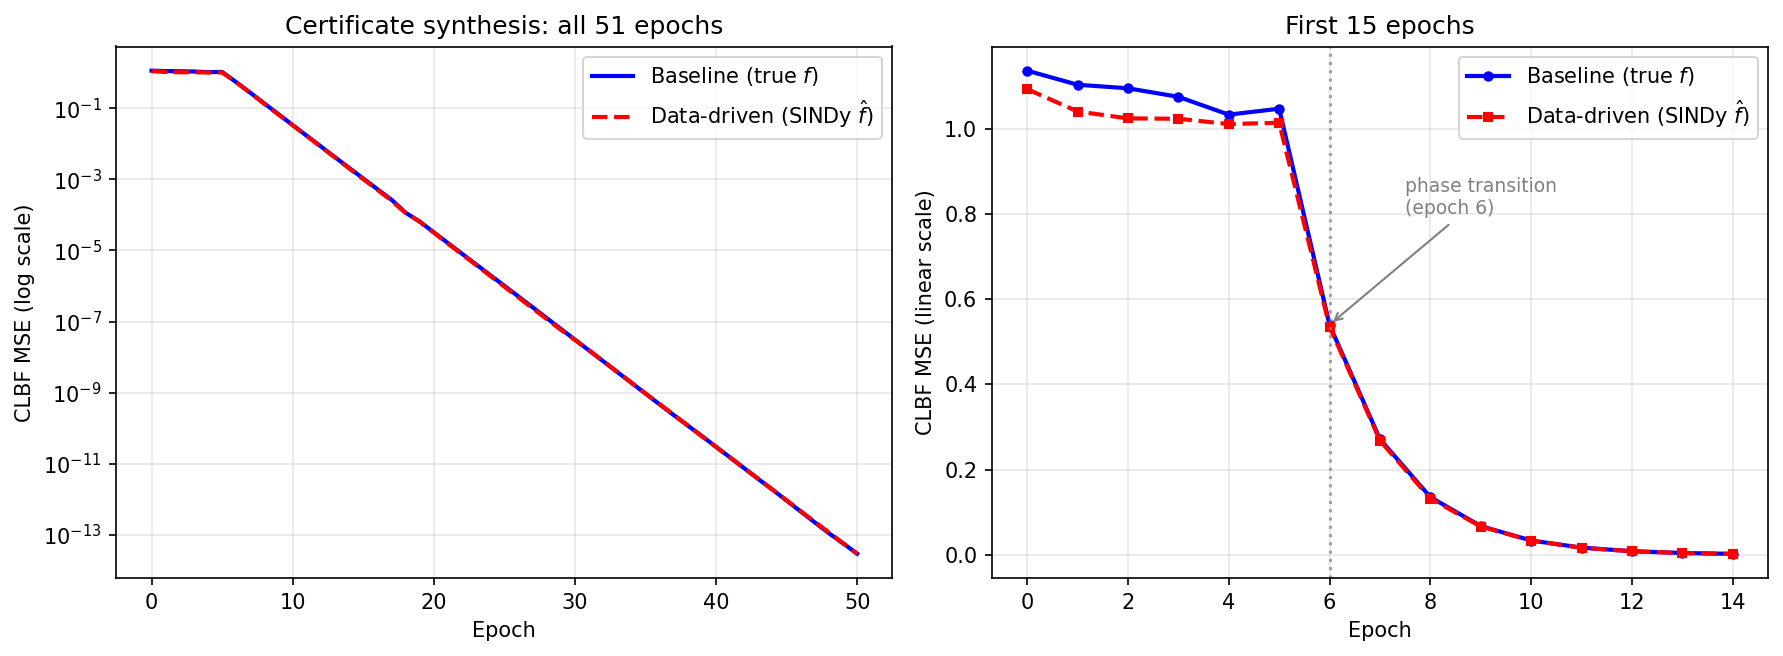
\includegraphics[width=0.95\linewidth]{clbf_comparison.png}
    \caption{Certificate synthesis under true versus learned dynamics on the
    inverted pendulum. \emph{Left:} CLBF MSE over all $51$ epochs (log scale).
    \emph{Right:} the first $15$ epochs (linear scale), with the phase transition
    at epoch $6$ marked. The trajectory trained against the SINDy estimate $\hf$
    (red, dashed) is nearly indistinguishable from the one trained against the
    true field $f$ (blue, solid): both undergo the same phase transition and
    converge to the same floor, empirically confirming the graceful-degradation
    prediction of Theorem~\ref{thm:main} for the small measured $\delta$.}
    \label{fig:clbf-comparison}
\end{figure}

\begin{table}[t]
    \centering
    \caption{CLBF MSE at representative epochs for the certificate trained against
    the true dynamics $f$ (baseline) and against the SINDy estimate $\hf$
    (data-driven). Both runs use $51$ epochs and $7191$ steps. The two curves
    track one another to within their step-to-step noise throughout training.}
    \label{tab:clbf-comparison}
    \begin{tabular}{lccc}
        \toprule
        & Epoch $0$ (init.) & Epoch $6$ (transition) & Epoch $50$ (final) \\
        \midrule
        Baseline (true $f$)        & $1.14$ & $0.54$ & $3.0\times10^{-14}$ \\
        Data-driven (SINDy $\hf$)  & $1.09$ & $0.54$ & $2.9\times10^{-14}$ \\
        \bottomrule
    \end{tabular}
\end{table}

Figure~\ref{fig:clbf-comparison} and Table~\ref{tab:clbf-comparison} summarize the
comparison. Three observations stand out. First, both pipelines exhibit the same
\emph{phase transition} at epoch $6$, where the CLBF MSE drops sharply from
$\mathcal{O}(1)$ as the network discovers a valid certificate structure. Second,
after the transition both losses decay at the same exponential rate and reach the
same numerical floor ($\approx 3\times10^{-14}$, i.e.\ machine-precision-limited)
by epoch $50$. Third, the largest gap between the two curves at any epoch is well
within the step-to-step training noise. In other words, learning the dynamics from
$20{,}000$ transitions cost essentially nothing in certificate quality: the
data-driven certificate is as valid as the one synthesized with exact physics.

This is the empirical content of Theorem~\ref{thm:main}. The measured dynamics
error over the operating region, $\delta\approx 0.049$, makes the predicted offset
$B\delta/\lambda_1$ negligible relative to the certificate scale, and the observed
training curves are correspondingly indistinguishable. The result substantiates
the paper's central claim: Lyapunov-guided diffusion control retains its safety
and stability guarantees when the dynamics are not known a priori but are instead
recovered from data by sparse identification.

\newpage

\bibliography{references}
\bibliographystyle{abbrvnat}

\end{document}